\chapter{Data Review}

In this chapter we take a deeper look into the data and the process of collecting, translating, and encoding the data. Our partner has provided a small sample of 1000 labeled data points. This data was manually labeled by an human annotator. 

\section{Overview}

The data consists of a merchant name, merchant website (url), merchant category, and merchant tag as shown in Table \ref{tab:data_point}. 

\begin{table}[h]
\begin{tabular}{|l|l|l|l|}
\hline
merchant name            & merchant url            & merchant category & merchant tags           \\ \hline
State Hospital & http://hospital.com/ & Health   & '\{"Clinic"\}' \\ \hline
\end{tabular}
\caption{This is an example of a single data point from the original data set.}
\label{tab:data_point}
\end{table}


The current process consists of giving the merchant url to an annotator. The annotator then views the website and either can instantly (after viewing the homepage) provide a label and tags for the website. However, in some cases the annotator may need to browse further (by viewing sibling pages such as the 'About Us' section or individual product pages) to get an idea of how the website should be classified. 

The annotator simply needs to view then mentally process the text and images from the website and make some reasonable decisions on how the site should be classified. However, the annotator does not record what the content on the site said or what drove them to make their decision.As a result we are missing a key portion of data for the classification process. 

Tags are also when labeling the data to provide further granularity. The merchant tags are ordered by specificity, with the first tag in the list being the most general and the final being the most specific. An example of the tag hierarchy is show in Table. \ref{tab:tags} where we can see that this sample consists of data from various categories all contained within the 'Eco' side tag grouping.


\begin{table}[h]
\begin{tabular}{|l|l|l|l|l|}
\hline
Category    & Level 1 Tag           & Level 2 Tag        & Level 3 Tag  & Side Tag \\ \hline
Travel      & Local Transport       & Micro-mobility     & Bike Sharing & Eco      \\ \hline
            &                       & Public Transport   &              & Eco      \\ \hline
Fashion     & Clothing - Other      & Second Hand        &              & Eco      \\ \hline
Car         & Charging Station      &                    &              & Eco      \\ \hline
            & Car Sharing           &                    &              & Eco      \\ \hline
\end{tabular}
\caption{This is an example of how the tags use different levels.}
\label{tab:tags}
\end{table}

The tags are important because they allow us to separate the data even further and group or sort the data differently. However, in our work we didn't opt to include the tags in the classification or selection strategy process at this time.

\section{Collection}

Similarly to the annotator our goal is to automate the navigation, collection/ storing process, and classification of the website. This speeds up the browsing process by navigating to websites that have already been labeled and scraping the text data and storing it into a database. We also make the obvious checks to see if the website has already been scraped and stored in the database to ensure we are not wasting time and resources.

The initial 1000 data points we received were labels with a pointer (a url) to where the text data is located (the website). The labels needed to be augmented with the text from the websites. For the human annotator, this text data is stored is simply stored in their short term memory while they view the website. Once they have a category for the website they can mostly forget about the text data and move on to assigning a category to the next website.

To gather the text data from the websites we used the Scrapy framework to extract text data from a single top level page of a website. We chose only to scrape the top level (main or home) page text because of the results published in another study where it was observed that adding more pages to the data set does not necessarily mean obtaining better results (\cite{sahid2019ecommerce}). 

Out of these initial data points 184 contained links that could not be accessed or links that provided no text data that could be scraped. Two websites were particularly problematic. Facebook and Instagram both are used by businesses as main information webpages. However, neither site allows for simple text scraping and a more advanced approach was needed to extract data from business with information on these platforms. In an effort to reduce the complexity of our scraper we decided to not create an additional scraper or integrate an API to handle these websites. Out of the remaining 816 data points 275 of them were in English. Out of the remaining 275 English data points the data was distributed into the categories as shown in Figure \ref{fig:original_english_counts}.

Our goal was to see how well the classifier and active learning sampling strategies would perform with limited data, but 275 samples with 23 categories was a bit to small and we still had a significant amount of data that wasn't being used (i.e. the untranslated data) so we decided we needed to find a way to translate the existing data. We tried various libraries available on GitHub but weren't getting good consistent results and we were hitting API request limits. After some time, we found that Azure had a service available and a free option of up to 2 million characters translated per month. This was a viable option and we were able to use this API to translate the remaining data. We limited the number of characters to 1000 per non English data point from the scraped text to avoid maxing out the API.

\section{Processing}

It is important for us to have the data in English as it allows us to exploit stop words when using the Scikit-Learn TF-IDF vectorizer to construct our data set. Stop words are words like “and”, “the”, “him”, which are presumed to be uninformative in representing the content of a text, and which may be removed to avoid them being construed as signal for prediction (\cite{sklearn62feature}). This holds true for our data set as well because we are not analyzing the text for sentiment or other linguistic features. We are simply looking for the most common words in each category.

At this stage, it was clear that our data set wasn't representing all categories equally. The 'Food and Drink' category has many more data points then the 'Culture' and 'Investments' categories which each had a single data point, see Figure \ref{fig:original_english_counts}. The 'Children' and 'Financial Services' categories weren't represented at all. Obviously this was problematic because we would like to have, minimum, three data points in each category to build train and test sets.

\begin{figure}[!ht]
  \centering
  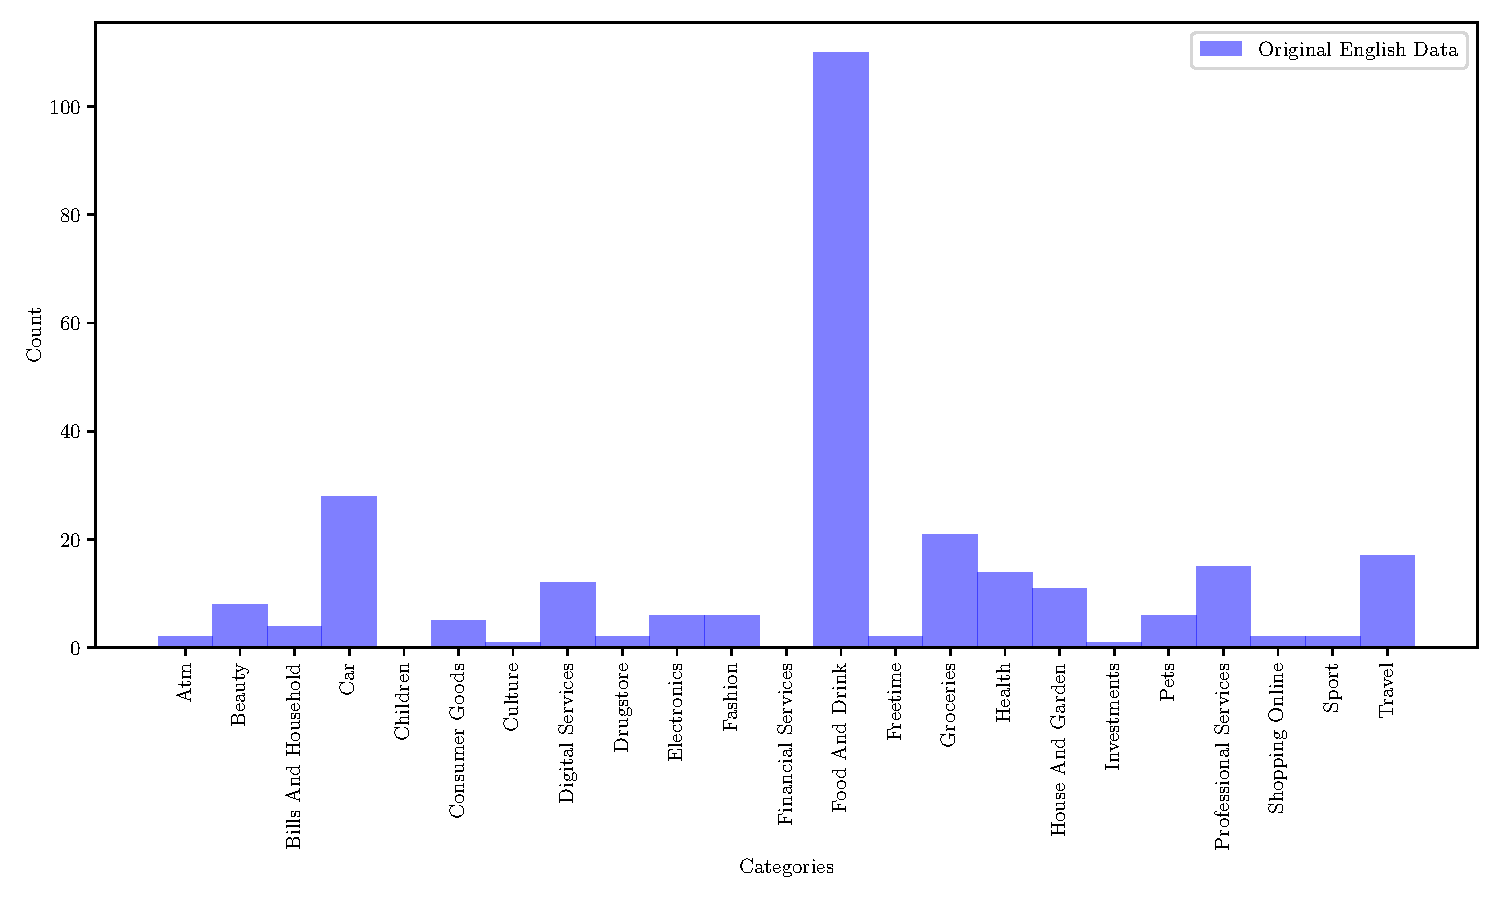
\includegraphics[width=\textwidth]{../img/plot_original_english_counts.pdf}
  \caption{The histograms for the original usable english data.}
  \label{fig:original_english_counts}
\end{figure}

An example of the first 100 characters of raw scraped text data from a website is shown in Table \ref{tab:text_examples}. The scraped text data is a single string of text that is a concatenation of all the text data pulled from the website url. 

\begin{table}[!ht]
\centering
\caption{Raw text collected by scraper and the translated text.}
\begin{tabular}{|l|p{10cm}|}
\hline
Raw & DentalVision - Profesionální soukromá zubní klinika v centru Hradce Králové ÚvodSlužby a ceníkOrdina \\ \hline
Translated & DentalVision Professional private dental clinic in the center of Hradec Králové IntroductionServices \\ \hline
\end{tabular}
\label{tab:text_examples}
\end{table}

We can see that html and other symbols are removed and the majority of the words were translated. There are still some issues with words being concatenated such as 'IntroductionServices' however we do try to separate these words after translation using a regex pattern, but we attempt to break these words apart before passing the text to the TF-IDF vectorizer.

To complement the original data we manually collected and labeled 141 additional data points for the categories that had low representation. This consisted of searching the internet for lists of websites similar to the ones in each category. Next we would browse the site to see if it was relevant and then add it to our list of additional websites and provide it a label. This was necessary because some categories only had 2 or 3 samples, however it was quite time consuming. The additional data are almost all from English language websites, this made it easier for us to explore and provide accurate labels for the sites. These data group splits will be referenced in the following experiments and a table of the exact counts for each group can be found in Appendix Table \ref{tab:data_counts}. In Figure \ref{fig:all_hist}. we show a bar chart of the counts of the original data and the additional data for each category and for each language, with the two letter language codes used to represent the languages.

\begin{figure}[!ht]
  \centering
  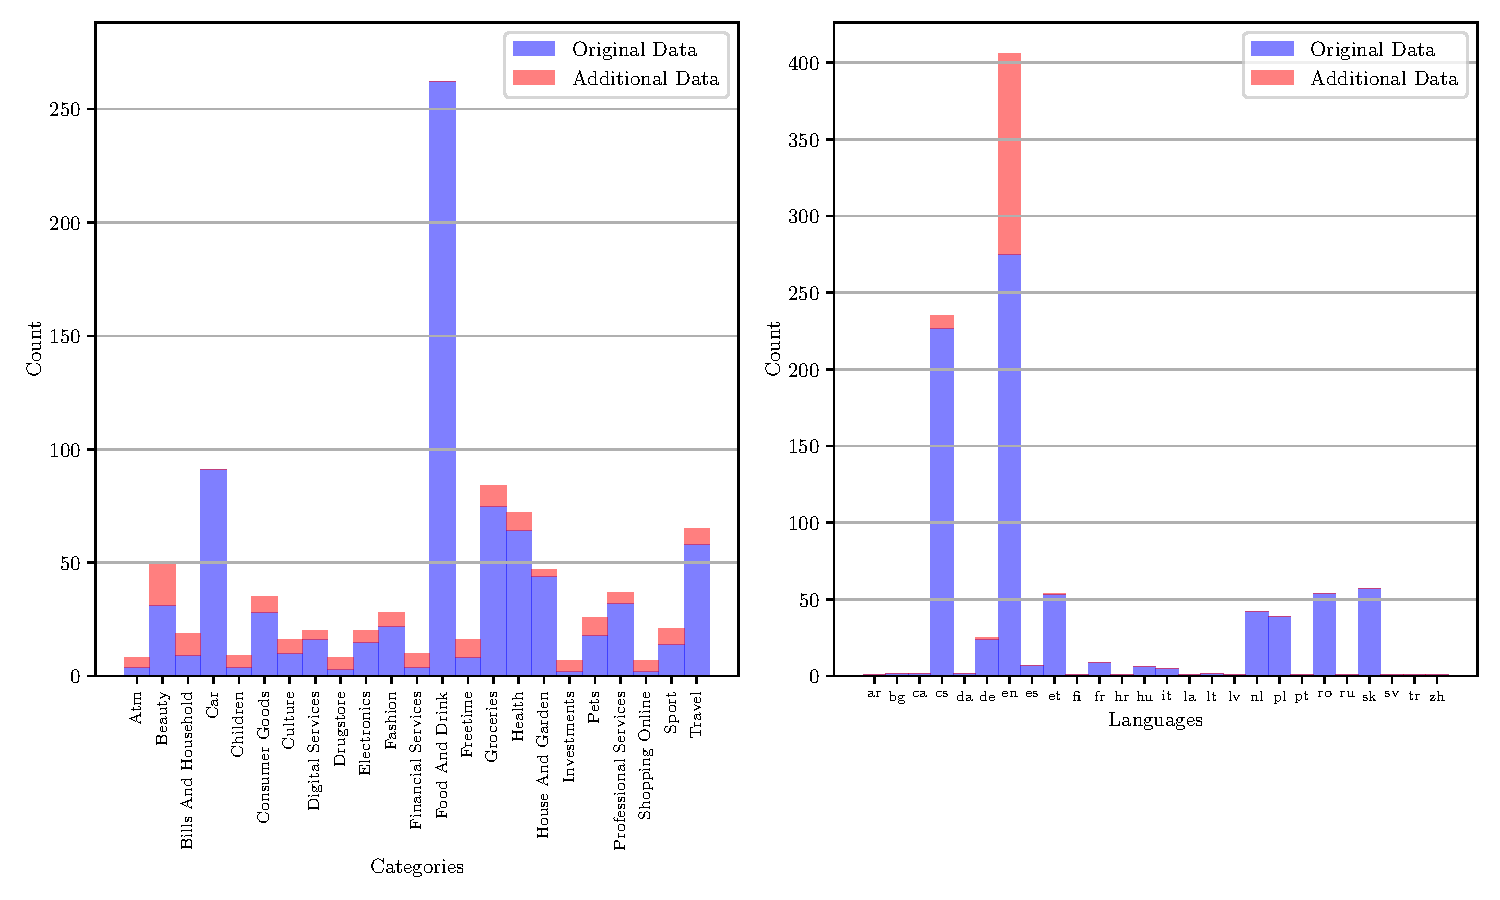
\includegraphics[width=\textwidth]{../img/plot_all_hist.pdf}
  \caption{The histograms for the original and additional data for all languages.}
  \label{fig:all_hist}
\end{figure}


After translating the data we used the TF-IDF vectorizer from Scikit-Learn. TF-IDF is an important tool commonly used in natural language processing and data science. The first part, TF, stands for term frequency and is a measure of how often a term appears in a document, while IDF (inverse document frequency) is a measure of how important a term is in a set of documents. The idea behind IDF is that a term that appears in many documents is less important than a term that appears in only a few documents, as the former is likely to be more common and less discriminative. The formula for calculating TF-IDF is as follows:

\begin{equation}
    \text{TF-IDF} = TF \times IDF
    \label{eq:tfidf}
\end{equation}

where:

\begin{flalign*}
    \text{TF} &= \frac{\text{number of occurrences of term $t$ in document}}{\text{total number of terms in document}} \\
    \text{IDF} &= \log_{e}(\frac{\text{total number of documents}}{\text{number of documents with term $t$ in it}})
\end{flalign*}

To calculate the TF-IDF score for a given term in a document, we would first calculate the term frequency (TF) by counting the number of times the term appears in the document and dividing it by the total number of terms in the document. Then, we would calculate the inverse document frequency (IDF) by taking the logarithm of the total number of documents in the set divided by the number of documents that contain the term. Finally, we would multiply TF by IDF to get the TF-IDF score for the term in the document as shown in Equation \ref{eq:tfidf}.

This process is repeated for each term in each document in the corpus, resulting in a TF-IDF matrix that can be used for various natural language processing tasks such as text classification, information retrieval, and clustering. It is important to understand TF-IDF because it is the basis for the feature selection we use throughout our experiments.

We were also able to find highly correlated words for each category using chi-squared analysis with all useable data, shown below in Table \ref{tab:correlated_unigrams_original}. Chi-squared analysis is a statistical method used to determine the association between two categorical variables. It is used to test whether two categorical variables are independent of each other or not. In other words, it helps to determine if there is a significant relationship between two variables.

The chi-squared test involves comparing the observed frequencies of each category in a contingency table to the expected frequencies. A contingency table is a two-dimensional table that shows the frequency distribution of two categorical variables. The expected frequencies are the frequencies that would be expected if the two variables were independent. The difference between the observed and expected frequencies is then squared, divided by the expected frequency, and summed over all categories to give the chi-squared statistic. The formula for calculating the chi-squared statistic is as follows:

\begin{equation}
    \chi^2 = \sum \frac{(O_i - E_i)^2}{E_i}
\end{equation}

where:

\begin{flalign*}
    \chi^2 &= \text{the chi-squared statistic} \\
    O_i &= \text{the observed frequency of category i} \\
    E_i &= \text{the expected frequency of category i}
\end{flalign*}

The degrees of freedom for the chi-squared test are calculated as (number of rows - 1) x (number of columns - 1). The chi-squared statistic is then compared to a critical value from a chi-squared distribution table with the degrees of freedom and a specified level of significance. If the calculated chi-squared statistic is greater than the critical value, then we reject the null hypothesis that the two variables are independent.

Some categories such as 'Culture', 'Digital Services', 'Shopping Online' that have few data points have words such as 'kihnu', 'synnex', 'joom', respectively, which have no relative meaning to the category in English but also show the limitations of our website scraping and translation capabilities. We also have the problem where some words are actually important but weren't translated correctly such as 'maso' in the 'Groceries' category, which means 'meat' in Czech but wasn't translated properly.

From what we discussed in the previous section, we can see that the 'Culture' category has only one data point and the 'Digital Services' category has only two data points. This is problematic because if the single data point we have doesn't represent the category well then we will continue to have difficulty classifying until we have more robust data.


\begin{table}[!ht]
\centering
\caption{Keywords from TF-IDF with chi-squared using the original data.}
\begin{tabular}{llll}
\toprule
{} &       Keyword 1 &      Keyword 2 &   Keyword 3 \\
\midrule
Atm                   &         banking &    individuals &       caixa \\
Beauty                &    hairdressing &    hairdresser &        hair \\
Bills And Household   &         liberty &       internet &    fullness \\
Car                   &            cars &           auto &         car \\
Children              &             toy &           sold &     toysrus \\
Consumer Goods        &           kiosk &        flowers &      flower \\
Culture               &         theater &         museum &       kihnu \\
Digital Services      &          synnex &          bitly &     servers \\
Drugstore             &     esodrogeria &      detergent &     drimble \\
Electronics           &         laptops &          onoff &   computers \\
Fashion               &           rings &      jewellery &       women \\
Financial Services    &             pre &         nissan &   insurance \\
Food And Drink        &            cafe &            bar &  restaurant \\
Freetime              &  representation &         casino &      likely \\
Groceries             &          liquor &           maso &      bakery \\
Health                &            drug &         dental &    pharmacy \\
House And Garden      &       skylights &         paints &    hardware \\
Investments           &        mistakes &     investment &      patria \\
Pets                  &             mat &            pet &  veterinary \\
Professional Services &          toilet &        faculty &      parcel \\
Shopping Online       &           owner &        default &        joom \\
Sport                 &          adidas &      singltrek &  functional \\
Travel                &           rooms &  accommodation &       hotel \\
\bottomrule
\end{tabular}

\label{tab:correlated_unigrams_original}
\end{table}

We also calculated the variable importance using the RandomForestRegressor from Scikit-Learn and provided a list of the top 20 most important words from the TF-IDF vectorizer. This helps orient ourselves within the data and check if there may be any major anomalies. This list can be found in Appendix Table \ref{tab:top_20_words}.

